%%%%%%%%%%%%%%%%%%%%%%%%%%%%%%%%%%%%%%%%%%%%%%%%%%%%%%%%%%%%%%%%%%%%%%%%%%%%%%%%
%%%%%%%%%%%%%%%%%%%%%%%%%%%%%%%%%%%%%%%%%%%%%%%%%%%%%%%%%%%%%%%%%%%%%%%%%%%%%%%%

\section{\textcolor{red}{Estágios da musicalidade na dança}}
\index{Musicalidade!Estágios da musicalidade}
\label{sec:aspectosusicalidade}
Quando estamos no percorrido de ter uma dança mais musical,
passamos por vários estágios de autoconhecimento e de aprendizagem; 
dependendo da relação que conscientemente nós tenhamos entre a música e o nosso corpo.
Neste sentido, vários dançarinos, professores e escritores,
propuseram formas de modelar por camadas ou estágios, a relação que existe entre a dança e a música.
Um desses modelos é indicado pelo dançarino e escritor Russell J. Hall,
que no seu blog ``Tango Words'', 
indica que podemos dançar no \hyperref[ref:Pulso]{\textbf{pulso}}, 
no \hyperref[sec:pos:Ritmo]{\textbf{ritmo}} ou na música \cite{TangoWordsEstagiosMusicalidade1}.
Por outro lado o dançarino de tango ``Paul Yang'' no seu blog ``In Search of Tango'',
ressalta que além de dançar no pulso e no ritmo, 
podemos  dançar na \hyperref[sec:pos:Melodia]{\textbf{melodia}} \cite{InSearchOfTangoEstagiosMusicalidade1}.
Em geral, podem ser achados em foros e blogs da internet,
muitas referencias e debates sobre estos estágios da musicalidade;
porem, é possível resumir todas essas ideias nos seguintes estágios da musicalidade.

\begin{description}
%%%
\item[Dançar no pulso:] (Ou dançar na \hyperref[def:Metrica]{\textbf{métrica}}) 
Dançar usando o \hyperref[ref:Pulso]{\textbf{pulso}}, 
implica nos movimentar com coerência com a música, 
utilizando como parâmetro de seguimento o pulso ou a métrica.
Por exemplo, se pensamos num passo com um ritmo ``rápido rápido lento'',
encaixamos ele dentro do compasso da música (métrica), e continuamos usando este movimento,
aconteça o que aconteça na peça musical;
então estaremos só dançando no pulso.
%%%
\item[Dançar no ritmo:] Dançar usando o \hyperref[sec:pos:Ritmo]{\textbf{ritmo}},
implica movimentar-nos com coerência com a música, 
utilizando como parâmetro de seguimento 
o ritmo em alguma linha melódica ou não melódica.
Por exemplo, se percebemos  um ritmo como: \Vier \Acht \Vier  \Acht \Vier \Halb,
e nossos movimentos são realizados seguindo ele, então estamos dançando no ritmo.
É importante ressaltar, que o ritmo na música tem em conta a métrica,
pelo que se dançamos no ritmo também estamos dançando no \hyperref[ref:Pulso]{\textbf{pulso}}.  
%%%
\item[Dançar na melodia:] Dançar usando a \hyperref[sec:pos:Melodia]{\textbf{melodia}},
implica algo mais que movimentar-nos seguindo variações de tempo (ritmo); 
pois na melodia se encontram as componentes \hyperref[ref:emotionsentimental]{\textbf{emocional}} 
e \hyperref[ref:emotionsentimental]{\textbf{sentimental}}, junto com a beleza, fluides, entre outros; 
que podemos perceber numa peça musical.
É claro que todas estas percepções subjetivas, 
são gerados por aspectos da melodia como: a articulação, cadencias, ritmos, consonâncias, dissonâncias,
variações de intensidade, etc. 
Pelo que se o dançarino interpreta a informação de todos estes aspectos,
estaria sim dançando com a melodia.
É importante ressaltar, que uma a melodia na música tem em conta o ritmo e a métrica,
pelo que se dançamos na melodia também estamos dançando no \hyperref[sec:pos:Ritmo]{\textbf{ritmo}} e
no \hyperref[ref:Pulso]{\textbf{pulso}}.
%%%
\item[Dançar na música:] 
Dançar usando a música implica movimentar-nos com coerência, 
seguindo os aspectos perceptíveis da música como, a métrica, 
o ritmo as variações de tons, tensão, articulação, etc.
Usando o fraseio e a interação entre distintas linhas melódicas;
de modo que possamos escolher informação de qualquer linha melódica ou acompanhamento,
e usar estes elementos em simultâneo.
Assim, seguindo esta descrição percebemos que dançar na música, 
implica que também se está dançando na \hyperref[sec:pos:Melodia]{\textbf{melodia}}, 
no \hyperref[sec:pos:Ritmo]{\textbf{ritmo}} e 
no \hyperref[ref:Pulso]{\textbf{pulso}}.
\end{description}~


Definidos estos estágios, 
devemos ressaltar que estos descrevem um processo que acontece por camadas;
é dizer que cada novo estagio do conhecimento cobre o anterior, formando um novo todo,
como é mostrado na Figura \ref{fig:aspectos-musica}.
\begin{figure}[h!]
    \centering
    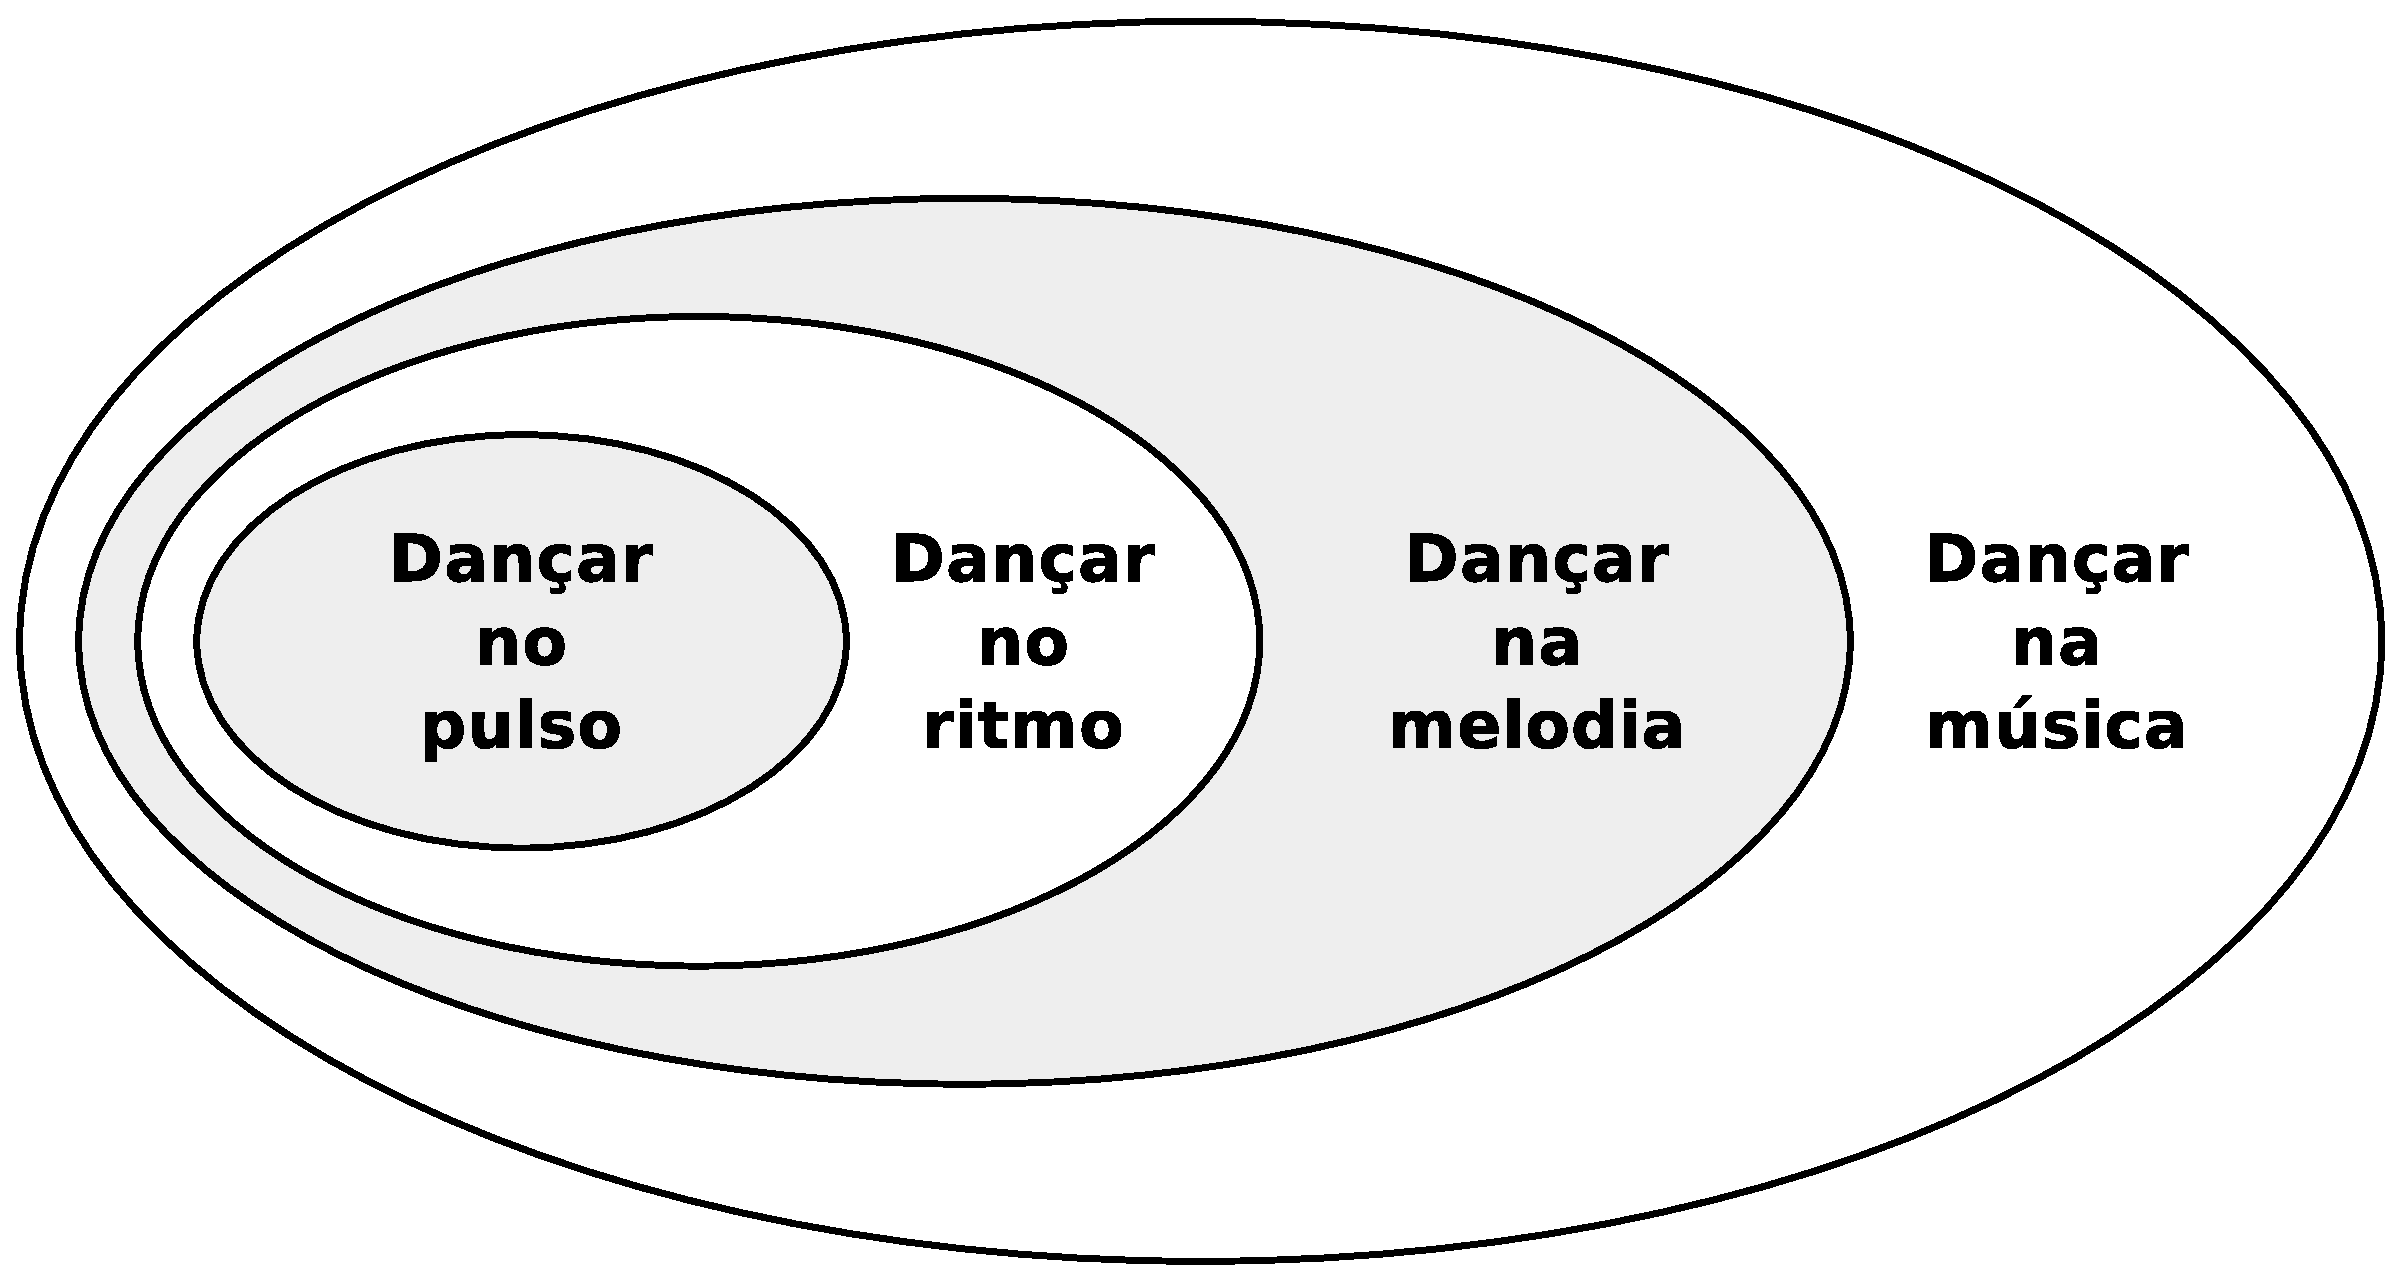
\includegraphics[width=\textwidth]{chapters/cap-musicalidade-tecnica/aspectos-musica.eps}
    \caption{Estágios da musicalidade na dança.}
    \label{fig:aspectos-musica}
\end{figure}


Nas seguintes seções para poder exemplificar os distintos estágios da musicalidade,
usaremos a composição musical titulada ``Lamento e consolo'',
cuja pauta é mostrada na Figura \ref{fig:lamento-e-consolo}.
Esta composição está liberada baixo a 
\hyperref[ref:licensalivre]{\textbf{licença livre}}:
\hyperref[subsec:CCBYSA]{\textbf{CC BY-SA}}.

\begin{sidewaysfigure}
    \centering
    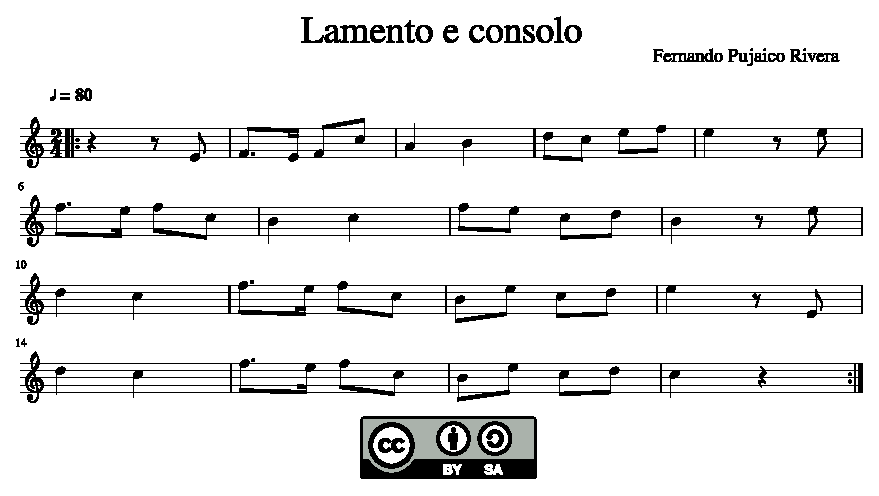
\includegraphics[width=\textwidth]{chapters/cap-musicalidade-tecnica/lamento-e-consolo-1.eps}
    \caption{Estágios da musicalidade na dança.}
    \label{fig:lamento-e-consolo}
\end{sidewaysfigure}

\begin{elaboracion}[title=Pausa ativa, width= 1.0\linewidth]
\index{Musicalidade!Pausa ativa}
\label{ref:pausaativa}
Em muitos momentos de nossa dança, como quando estamos seguindo uma linha melódica,
ou algum instrumento em particular, necessitamos realizar pausas, 
já seja porque acontece um breque na música, um final de frase musical ou algum outro evento.
Para estos casos, é recomendado realizar \textbf{pausas ativas}; é dizer,
permanecer com a mente atenta à música e a nosso entorno, 
mantendo em nosso corpo um tom muscular ativo\footnote{Não 
esquecendo a postura no abraço de dança se estamos dançando a dois. }, 
para estar prontos para sair quando se reinicie a melodia.

Também, para manter a métrica da música na nossa mente,
se for necessário, 
podemos realizar leves movimentos com alguma parte de nosso corpo (cabeça, ombros, quadril, etc.);  
de modo que poderemos souber quando iniciará o próximo tempo forte ou fraco.
Isto é importante para poder projetar o tempo de reinicio de nossa dança.
\end{elaboracion}


%%%%%%%%%%%%%%%%%%%%%%%%%%%%%%%%%%%%%%%%%%%%%%%%%%%%%%%%%%%%%%%%%%%%%%%%%%%%%%%%
%%%%%%%%%%%%%%%%%%%%%%%%%%%%%%%%%%%%%%%%%%%%%%%%%%%%%%%%%%%%%%%%%%%%%%%%%%%%%%%%
\subsection{Dançar no pulso}
\label{subsec:dancapulso}
\index{Musicalidade!Dançar no pulso}
Dançar no \hyperref[subsec:perpulsomusica]{\textbf{pulso}}\footnote{O 
tema de perceber o pulso musical é estudado na Seção \ref{subsec:perpulsomusica}.} 
pode também ser entendido como dançar na 
\hyperref[sec:percepcionmetrica]{\textbf{métrica}}\footnote{O 
tema de perceber a métrica na musica é estudado na Seção 
\ref{sec:percepcionmetrica}.},
pois dançamos tendo como única referencia o pulso
e o \hyperref[subsec:perceberTF1]{\textbf{tempo forte}}\footnote{O 
tema de perceber o tempo forte na musica é estudado na Seção 
\ref{subsec:perceberTF1}.} do compasso,
componentes indispensáveis para definir a métrica na música.

Assim, dado que estes aspectos, 
são os primeiros que aprendemos a reconhecer na música,
já seja de forma consciente ou inconsciente,
seu uso é considerado o primeiro estagio da musicalidade na nossa dança.
 
\begin{example}[Dançando executando ``tchic tchic tum'':]
\label{ex:dance:pulso}
Imaginemos que temos decidido executar nossos movimentos (ex: pisadas, ou movimentos de ombros, cabeça quadril, etc.),
seguindo uma distribuição de tempos ``tchic tchic tum'',
o que é equivalente a indicar que usaremos uma sequencia ``rápido rápido lento''.

Uma possível alternativa, para dançar no pulso, 
seria:
\begin{itemize} 
\item Encaixar o ``tchic tchic tum'', 
de maneira que esta distribuição de tempos encha completamente um compasso.
\item Decidindo  que o ``tum'', 
que consideramos o movimento principal da sequencia,
seja executado no tempo forte.
\end{itemize}

Seguindo estas considerações criativas,
nossa dança, 
usando a melodia ``Lamento e consolo'' (ver Figura \ref{fig:lamento-e-consolo}), 
estaria descrita como indica a Figura \ref{fig:lamentoconsolopulso1};
onde a melodia que escutamos está sendo executada por um ``bandolim'',
e as ``claves'' representam o ritmo que seguem nossos movimentos;
nesse caso foram escolhidos pisadas, como movimentos de exemplo.
É fácil perceber, nessa representação, 
como nossos movimentos usam pouco da informação que contem a melodia, 
pois a única caraterista que compartem é a métrica.
\end{example}
\begin{sidewaysfigure}
    \centering
    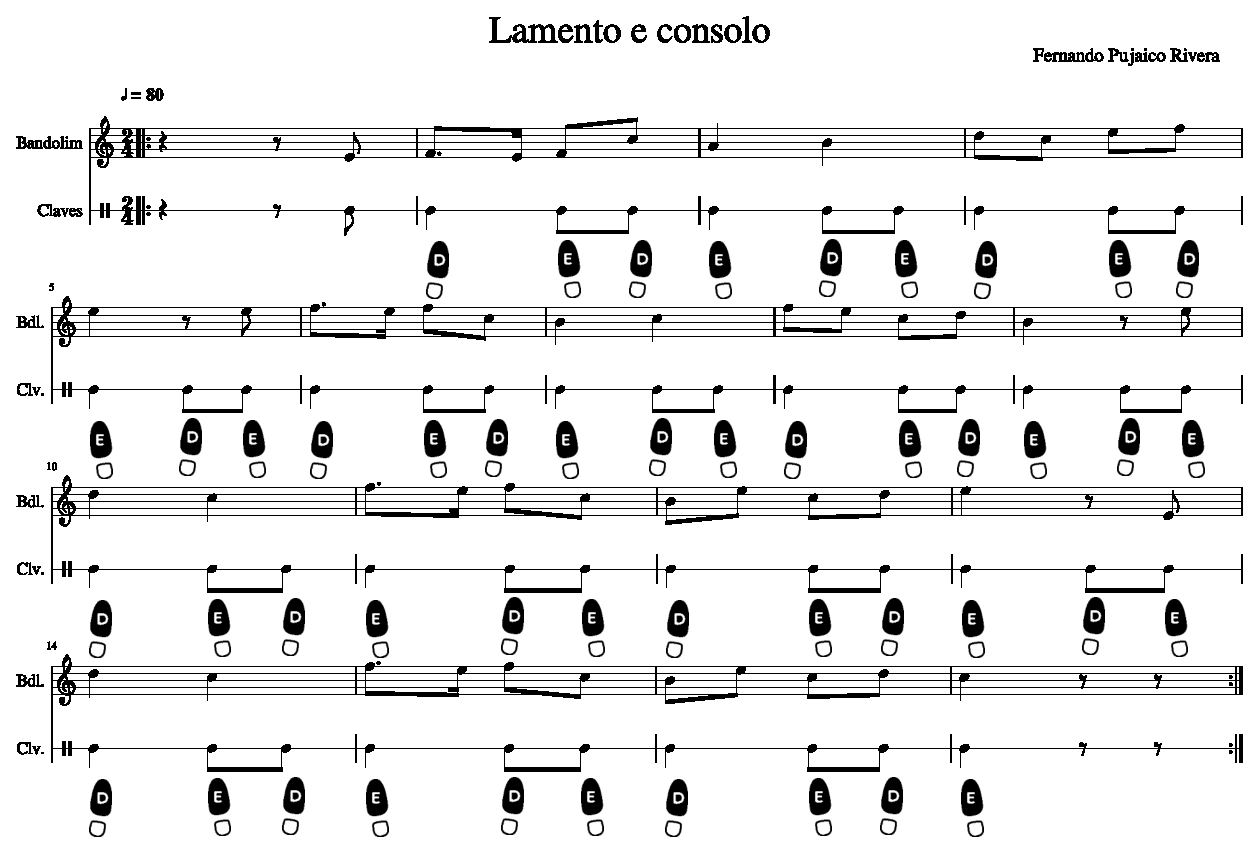
\includegraphics[width=\textwidth]{chapters/cap-musicalidade-tecnica/lamento-e-consolo-clave-pulso-1.eps}
    \caption{Música dançada no pulso.}
    \label{fig:lamentoconsolopulso1}
\end{sidewaysfigure}

\subsubsection{Forma evoluída de dançar no pulso ou diminuída de dançar no ritmo?}
Um caso interessante, é quando apos ter aprendido a dançar no pulso,
ganhamos consciência da música e iniciamos a prestar atenção a outros aspectos além da métrica;
percebendo detalhes como o \hyperref[sec:perceberfrases]{\textbf{final de uma frase}} rítmica, 
ou os \hyperref[sec:percepcionbreak]{\textbf{breaks}} da  música.
Nesse momento, estamos usando informação extraída das frases rítmicas, 
pelo que estritamente falando estaríamos sim,  dançando no ritmo; 
porem, dado que a maior parte do tempo dançaríamos no pulso,
 poderíamos sentir que só estamos dançando uma forma evoluída de dançar no pulso.

\begin{example}[Dançando executando ``tchic tchic tum'' e breques:]
Se usamos as mesmas escolhas criativas que as vistas no Exemplo \ref{ex:dance:pulso},
e além disso agregamos que usaremos as pausas, ao final das frases rítmicas,
 na melodia ``Lamento e consolo'' (ver Figura \ref{fig:lamento-e-consolo}). 
Então estaríamos movimentando-nos como indica a Figura \ref{fig:lamentoconsolopulsobreak1};
onde similarmente ao Exemplo \ref{ex:dance:pulso},
as ``claves'' representam o ritmo que seguem nossos movimentos,
neste caso exemplificado com pisadas.

É fácil perceber, nessa representação, 
como nossos movimentos usam pouco da informação que contem a melodia, 
pois as únicas carateristas que compartem, movimento e música, 
são a métrica e o acompanhamento do final de frase rítmica.
Um ponto interessante a ressaltar,
 é que se na nossa tentativa de dançar como na Figura \ref{fig:lamentoconsolopulsobreak1}, 
percebemos que temos problemas em manter, na nossa mente, a métrica durante as pausas; 
uma boa regra geral, especialmente sim somos novos na dança, 
seria realizando \hyperref[ref:pausaativa]{\textbf{pausas ativas}};
é dizer, manter a métrica da música, neste caso binária, usando alguma parte de nosso corpo.
Por exemplo, poderíamos movimentar a cabeça, os ombros, o quadril, etc.
Acompanhando mentalmente o compasso binário,
deixando um pé livre, pronto para sair no próximo tempo forte com som.
\end{example}
\begin{sidewaysfigure}
    \centering
    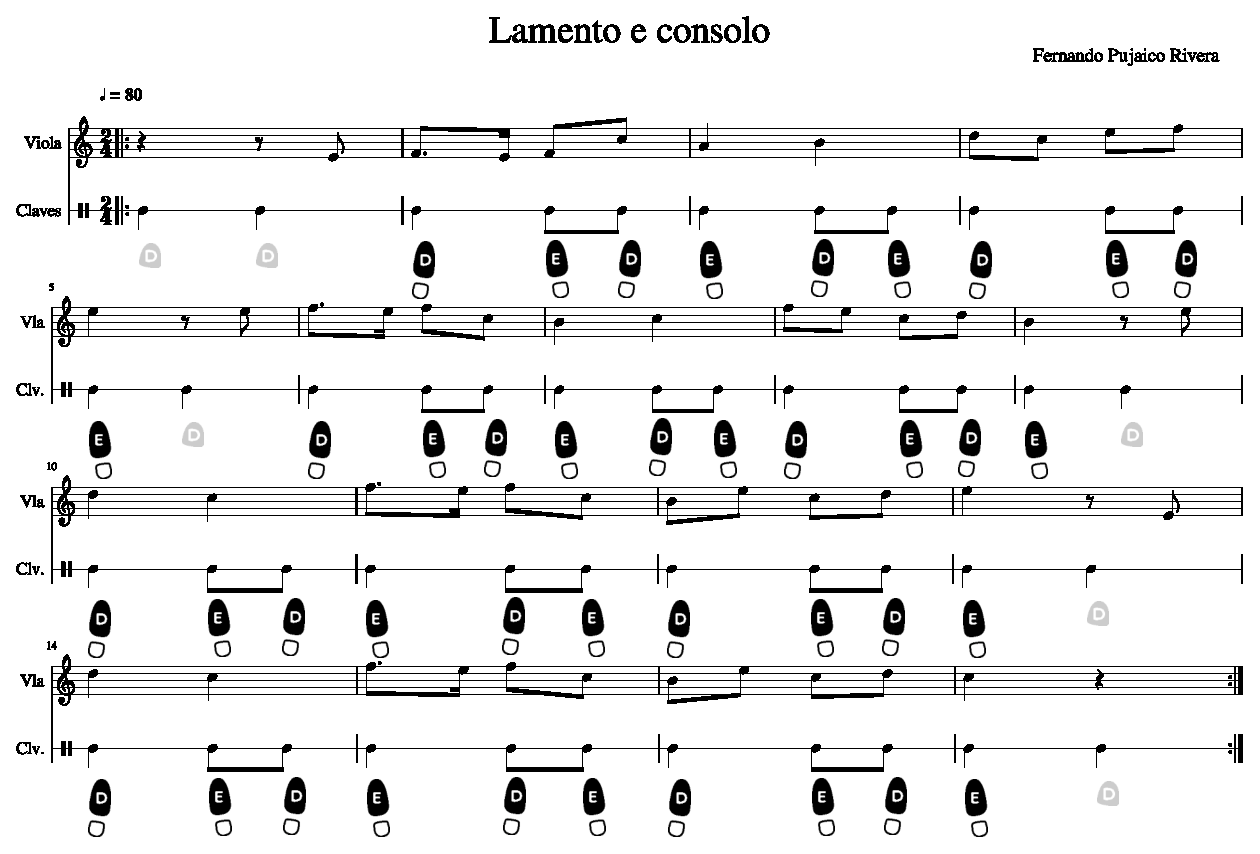
\includegraphics[width=\textwidth]{chapters/cap-musicalidade-tecnica/lamento-e-consolo-clave-pulso+break-1.eps}
    \caption{Música dançada geralmente no pulso e usando breaks.}
    \label{fig:lamentoconsolopulsobreak1}
\end{sidewaysfigure}

%%%%%%%%%%%%%%%%%%%%%%%%%%%%%%%%%%%%%%%%%%%%%%%%%%%%%%%%%%%%%%%%%%%%%%%%%%%%%%%%
%%%%%%%%%%%%%%%%%%%%%%%%%%%%%%%%%%%%%%%%%%%%%%%%%%%%%%%%%%%%%%%%%%%%%%%%%%%%%%%%
\subsection{Dançar no ritmo}
\label{subsec:dancaritmo}
\index{Musicalidade!Dançar no ritmo}
 Dançar usando o \hyperref[sec:pos:Ritmo]{\textbf{ritmo}},
é o segundo estágio de nosso percorrido na musicalidade.
Para atingir a competência neste estagio, 
devemos aprender a aproveitar todas as informações encontradas 
no ritmo; provenientes da música como um todo, de alguma linha melódica ou acompanhamento.

No modo mais simples ou cru, poderíamos pensar no ritmo,
como um conjunto de \hyperref[sec:figurasmusicais]{\textbf{figuras musicais}} 
colocadas uma apos de outra, 
e aproveitar figura a figura este \hyperref[sec:elementosmusica]{\textbf{elemento da música}}.
Porem, ao igual que quando escutamos um discurso,
sabemos que este em essência é um conjunto de letras,
e poderíamos entender-lho estudando-o desde essa perspetiva;
para nós seres humanos, 
muitas vesses é mais fácil pensar sempre em macro que em micro,
ou seja em estruturas maiores como palavras ou frases, perguntas, respostas ou ordens, etc. 
De modo que nosso cérebro, em muitos casos, 
já está adaptado com soluciones prontas para atender estes problemas.

Antes de passar a descrever estruturas maiores, 
é importante lembrar elementos menores que podem ser aproveitadas na música.
Primeiro devemos lembrar que existem 4 \hyperref[sec:carateristasom]{\textbf{características do som}},
estas são: 
\begin{inparaitem}
\item o tom, 
\item a duração, 
\item o timbre e 
\item a intensidade.
\end{inparaitem}
Destas quatro só o tom não vai ser aproveitada se dançamos no ritmo;
porem podemos usar o timbre e a intensidade do som para mudar nossas 
\hyperref[sec:musicalidade:dinamicas]{\textbf{dinâmicas do movimento}};
já a duração poderia ser usada dançando o ritmo figura musical por figura,
movimentando-nos atrelados a esse elemento.

Por outro lado, a nível macro, temos  motivos e frases rítmicas,
que poderíamos aproveitar seguindo elas ou interpretando-as, 
com suas obvias consequência como o melhor aproveitamento das pausas, 
como nos finais de frase musical ou nos ``breaks'' da música,
ou mudanças de movimentos na mudança de frase.

Assim, quando percebemos o ritmo numa música, 
podemos sim usar este elemento da música, figura a figura; 
porem, devemos lembrar que temos outros aspectos do ritmo,
agrupadas em estruturas maiores e menos evidentes que podemos aproveitar.


\begin{example}[dançando no ritmo seguindo as figuras musicais:]
\label{ex:dancaritmo1}
Imaginemos que temos decidido executar nossos movimentos (ex: pisadas, ou movimentos de ombros, cabeça quadril, etc.),
seguindo o ritmo de uma camada numa peça musical.
Nesse caso, uma possível alternativa para dançar no ritmo, 
seria movimentar nosso corpo seguindo uma a uma as figuras musicais.

Assumindo esta  consideração criativa para nossos movimentos, 
podemos usar a melodia ``Lamento e consolo'' (ver Figura \ref{fig:lamento-e-consolo}),
para dançar no ritmo, 
de modo que nossos movimentos seriam executados como indica a Figura \ref{fig:lamentoconsoloritmo1}.
A melodia a dançar está representada por um ``bandolim'',
e as ``claves'' representam o ritmo que seguem nossos movimentos;
nesse caso foram escolhidos pisadas, como movimentos de exemplo.
É fácil perceber, nessa representação, 
como nossos movimentos estão atrelados ao ritmo na música,
e não a outras informações como o tom das notas musicais.
\end{example}
\begin{sidewaysfigure}
    \centering
    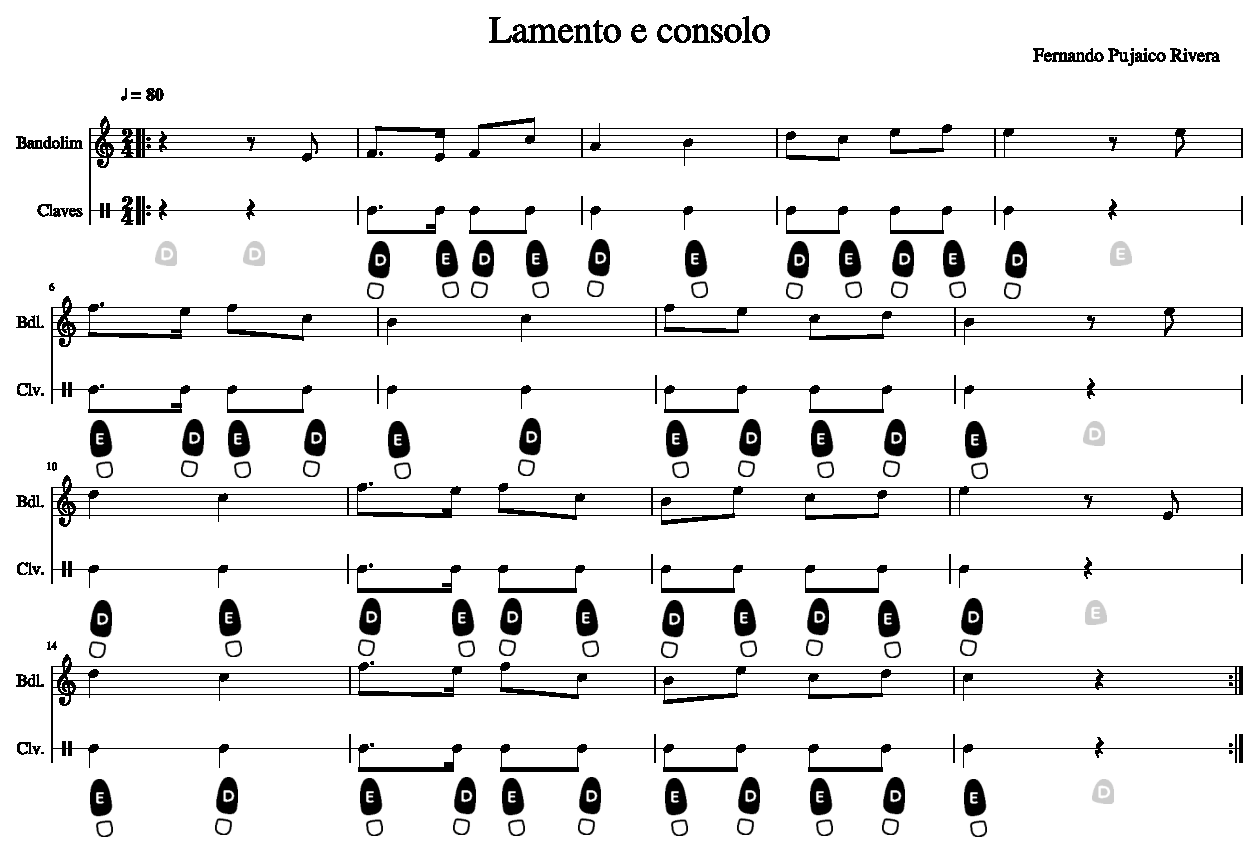
\includegraphics[width=\textwidth]{chapters/cap-musicalidade-tecnica/lamento-e-consolo-clave-ritmo-1.eps}
    \caption{Música dançada no ritmo.}
    \label{fig:lamentoconsoloritmo1}
\end{sidewaysfigure}


Neste quesito muitos professores e autores propuseram diferentes jeitos de aproveitar o ritmo; 
por exemplo, o dançarino e instrutor ``Andrew Sutton'', 
no seu blog sobre dança ``danceninjas'',
menciona na sua visão, alguns aspectos do ritmo que podem ser aproveitados \cite{AndrewSuttonRitmo1};
a seguir mostramos uma descrição destes conceitos.  
\begin{itemize}
%%%%%
\item Acertando o \hyperref[sec:Andamento]{\textbf{andamento}}:
Como já foi vista na Seção \ref{sec:Andamento},
o andamento é uma caraterística importante na música,
pois define o grau de lentidão ou rapidez ao executar,
uma peça musical. 
Dado que as figuras musicais, usadas para descrever um ritmo, 
só tem uma duração com valor relativo entre elas,
conhecer o andamento; é dizer, conhecer quantas batidas por minuto (BPM) tem cada figura musical,
nos ajudará a acertar qual deve ser a velocidade meia de nossa dança,
e predizer corretamente qual será a duração mínima e máxima da seguinte figura musical executada.
\begin{example}
Podemos perceber esta diferencia entre os andamentos, 
ao escutar a música ``Delírios de amor'' interpretada por ``Alcione'', 
de andamento lento, 
quanto comparado com a música ``vanerão sambado'' interpretado pelo grupo ``Os serranos'', 
com um andamento de maior rapidez.
De modo que para nos é evidente que em media nossos movimentos serão mais lentos,
no primeiro caso que no segundo.
\end{example}
%%%%%
\item Melhorando nosso \hyperref[sec:dancetimming]{\textbf{timing}}:
Este ponto já foi abordado na Seção \ref{sec:dancetimming},
onde se indica que ter a capacidade de ter o peso bem definido,
ao inicio de cada \hyperref[sec:TemposCoreograficos]{\textbf{tempo coreográfico}}, 
é muito importante esteticamente para projetar clareza em nossos movimentos,
e tecnicamente para poder ter o tempo completo entre movimentos consecutivos,
para poder executar \hyperref[sec:musicalidade:dinamicas]{\textbf{dinâmicas}}.
%%%%%
\item Seguindo as \hyperref[sec:figurasmusicais]{\textbf{figuras musicais}}:
A forma mais evidente de aproveitar o ritmo, 
é seguindo as figuras musicais com nossos movimentos;
assim, nesta tarefa podemos separar os ritmos percebidos em dois casos:
\begin{itemize} 
\item No primeiro, o ritmo que escolhemos tem uma caraterista cíclica ou regular,
aos quais denominaremos aqui como ritmos simples; podemos ver exemplos de ritmos simples,
no acompanhamento de uma linha melódica, 
pois geralmente estes repetem de forma cíclica uma frase rítmica curta.
\item No segundo caso, temos  ritmos compostos por figuras musicais,
com uma caraterista não cíclica num período longo de tempo; 
chamaremos a estos como ritmos complexos;
estes casos são vistos facilmente no ritmo da linha melódica principal de uma composição musical.
\end{itemize}
Mesmo que sejam dados exemplos específicos, 
indicando onde comumente poderemos achar ritmos simples e complexos;
na prática poderemos achar estes ritmos em qualquer camada de uma música,
ou pelo menos em uma seção dela; 
pois seus usos estão limitados só pela criatividade do compositor.
%%%%%
\item Usando \hyperref[sec:musicalidade:dinamicas]{\textbf{dinâmicas}} no ritmo: 
Uma forma de dar variedade e textura a nossos movimentos, 
é usando dinâmicas; este tema já foi tratado na Seção \ref{sec:musicalidade:dinamicas},
onde também estudamos os fatores do movimento.

Assim, algumas opções para trabalhar nosso ritmo usando dinâmicas, seriam:
\begin{itemize}
\item Aproveitar o \hyperref[sec:pos:timbre]{\textbf{timbre}} dos instrumentos que geram o ritmo,
para modelar nossas dinâmicas.
\begin{example}[Bumbo vs. pandeiro:]
quando seguimos  o ritmo executado pelo bumbo,
podemos fazer movimentos mais pesados ou com uma aparência de dançar num lugar com gravidade aumentada,
porem se o mesmo ritmo fosse executado por um pandeiro,
nossos movimento,
poderiam dar uma aparência de agilidade, 
como de algo que se movimenta ligeiramente.
\end{example}
\item Podemos também escolher uma porção do ritmo, como um motivo rítmico,
 ou o que consideremos ideias rítmica curtas,
é interpretar-lho com nossos movimentos seguindo alguma dinâmica.
\begin{example}[Usando motivos rítmicos:]
Damos passos pisando só a última figura musical de um motivo rítmico,
de modo que o movimento, para dar esse passo, pode ser rápido ou lento,
dependendo do juízo que façamos sobre o resto de figuras musicais do motivo.
Onde por exemplo, se são muitas figuras musicais de duração curta, 
faremos um movimento rápido para pisar a última figura;
e se as figuras musicais são poucas e de longa duração faremos um movimento lento.
\end{example}
\end{itemize}
\end{itemize}



%%%%%%%%%%%%%%%%%%%%%%%%%%%%%%%%%%%%%%%%%%%%%%%%%%%%%%%%%%%%%%%%%%%%%%%%%%%%%%%%
%%%%%%%%%%%%%%%%%%%%%%%%%%%%%%%%%%%%%%%%%%%%%%%%%%%%%%%%%%%%%%%%%%%%%%%%%%%%%%%%
\subsection{\textcolor{red}{Dançar na melodia}}
\label{subsec:dancamelodia}
\index{Musicalidade!Dançar na melodia}

Como já temos visto ate agora sobre os estágios da musicalidade, 
podemos \hyperref[subsec:dancapulso]{\textbf{dançar no pulso}}  ou no ritmo;
porem, quando escutamos uma música percebemos que esta não só contem ritmos estruturados, 
seguindo um acento \hyperref[def:Metrica]{\textbf{métrico}} com um \hyperref[sec:pos:timbre]{\textbf{timbre}} 
e uma \hyperref[sec:pos:Intensidade]{\textbf{intensidade}};
se não que também contem \hyperref[sec:pos:Melodia]{\textbf{melodias}} que são compostas, além de outros fatores, 
por mudanças de tons.
Conhecendo isto, 
podemos deduzir que para extrair mais atributos da música,
cuja interpretação nos leve a atingir diferentes estilos de dança,
podemos também nos concentrar no aproveitamento da melodia.


Porem, quando escutamos falar sobre dançar na melodia,
as pessoas não se referem geralmente a dançar interpretando as duas principais características de uma melodia,
que são as mudanças de \hyperref[sec:pos:Altura]{\textbf{tom}} e de
\hyperref[sec:pos:Duracion]{\textbf{duração}} nas figuras musicais;
e sim em interpretar estruturas ou aspectos mais complexos da melodia.


\begin{example}[Percebendo e estudando um poema:]
Para entender um poema poderíamos nos concentrar em estudar as letras, 
espaços em branco  e a posição destes no texto;
porem, estudar desta forma pode ser complexo para um ser humano,
que está acostumado a trabalhar pensando em macro estruturas e não em micro estruturas;
claro que a possibilidade de estudar um poema letra a letra existe,
porem não é isso o que a gente indica quando diz que quer estudar uma poesia.
Na forma mais mecânica, 
as pessoas poderiam se referir a estudar as palavras, as frases e sua função no texto;
também a forma em que as frases finalizam em rimas, a métrica,
a velocidade de leitura, entre outros fatores.
Além desta aproximação mais mecânica, 
poderíamos ascender na escala de complexidade e estudar formas ainda superiores de entender a poesia;
por exemplo, baseando-nos em aspectos mais subjetivos como, 
as emoções e sentimentos  que o texto desencadeia em nós;
ou tambem poderiamos estudar como o texto aumente e diminui a tensão em nós,
 com o uso adequado das palavras.
\end{example}

Da mesma forma que quando uma pessoa diz que vai estudar um poema, 
não se refere geralmente a estudar ele letra a letra;
quando indicamos que dançaremos na melodia,
não nos referiremos diretamente a dançar as mudanças de tom, 
e sim geralmente, se nossa visão da melodia é mais mecânica, a dançar interpretando os motivos, as frases,
o fraseio, as articulações, as cadencias, as formas estruturais, etc.
Por outro lado se procuramos uma visão e analises mais intimo da melodia,
poderíamos nos referir a interpretar com nossos movimentos, as emoções e sentimentos que a música acorda em nós;
ou poderíamos interpretar a tensão e relaxação que a melodia nos provoca,
também poderíamos incorporar na nossa dança o grau de fluidez ou descontinuidade na articulação das notas musicais, etc.

Assim, observamos que temos vários níveis, 
de onde poderemos extrair caracteristicas da melodia que possam ser interpretados em nossos movimentos;
a Figura \ref{fig:etapa-melodica-1} mostra de forma ordenada,
algumas características que podem ser extraídas da música, 
agrupados desde estruturas mais complexas (esquerda) a menos complexas (direita).
É importante ressaltar que alguns elementos destes grupos excedem a definição de melodia, como a textura, a harmonia, etc.
Estos aspectos serão tratados quando falemos sobre \hyperref[subsec:dancamusica]{\textbf{dançar na música}}.

\begin{figure}[!h]
    \centering
    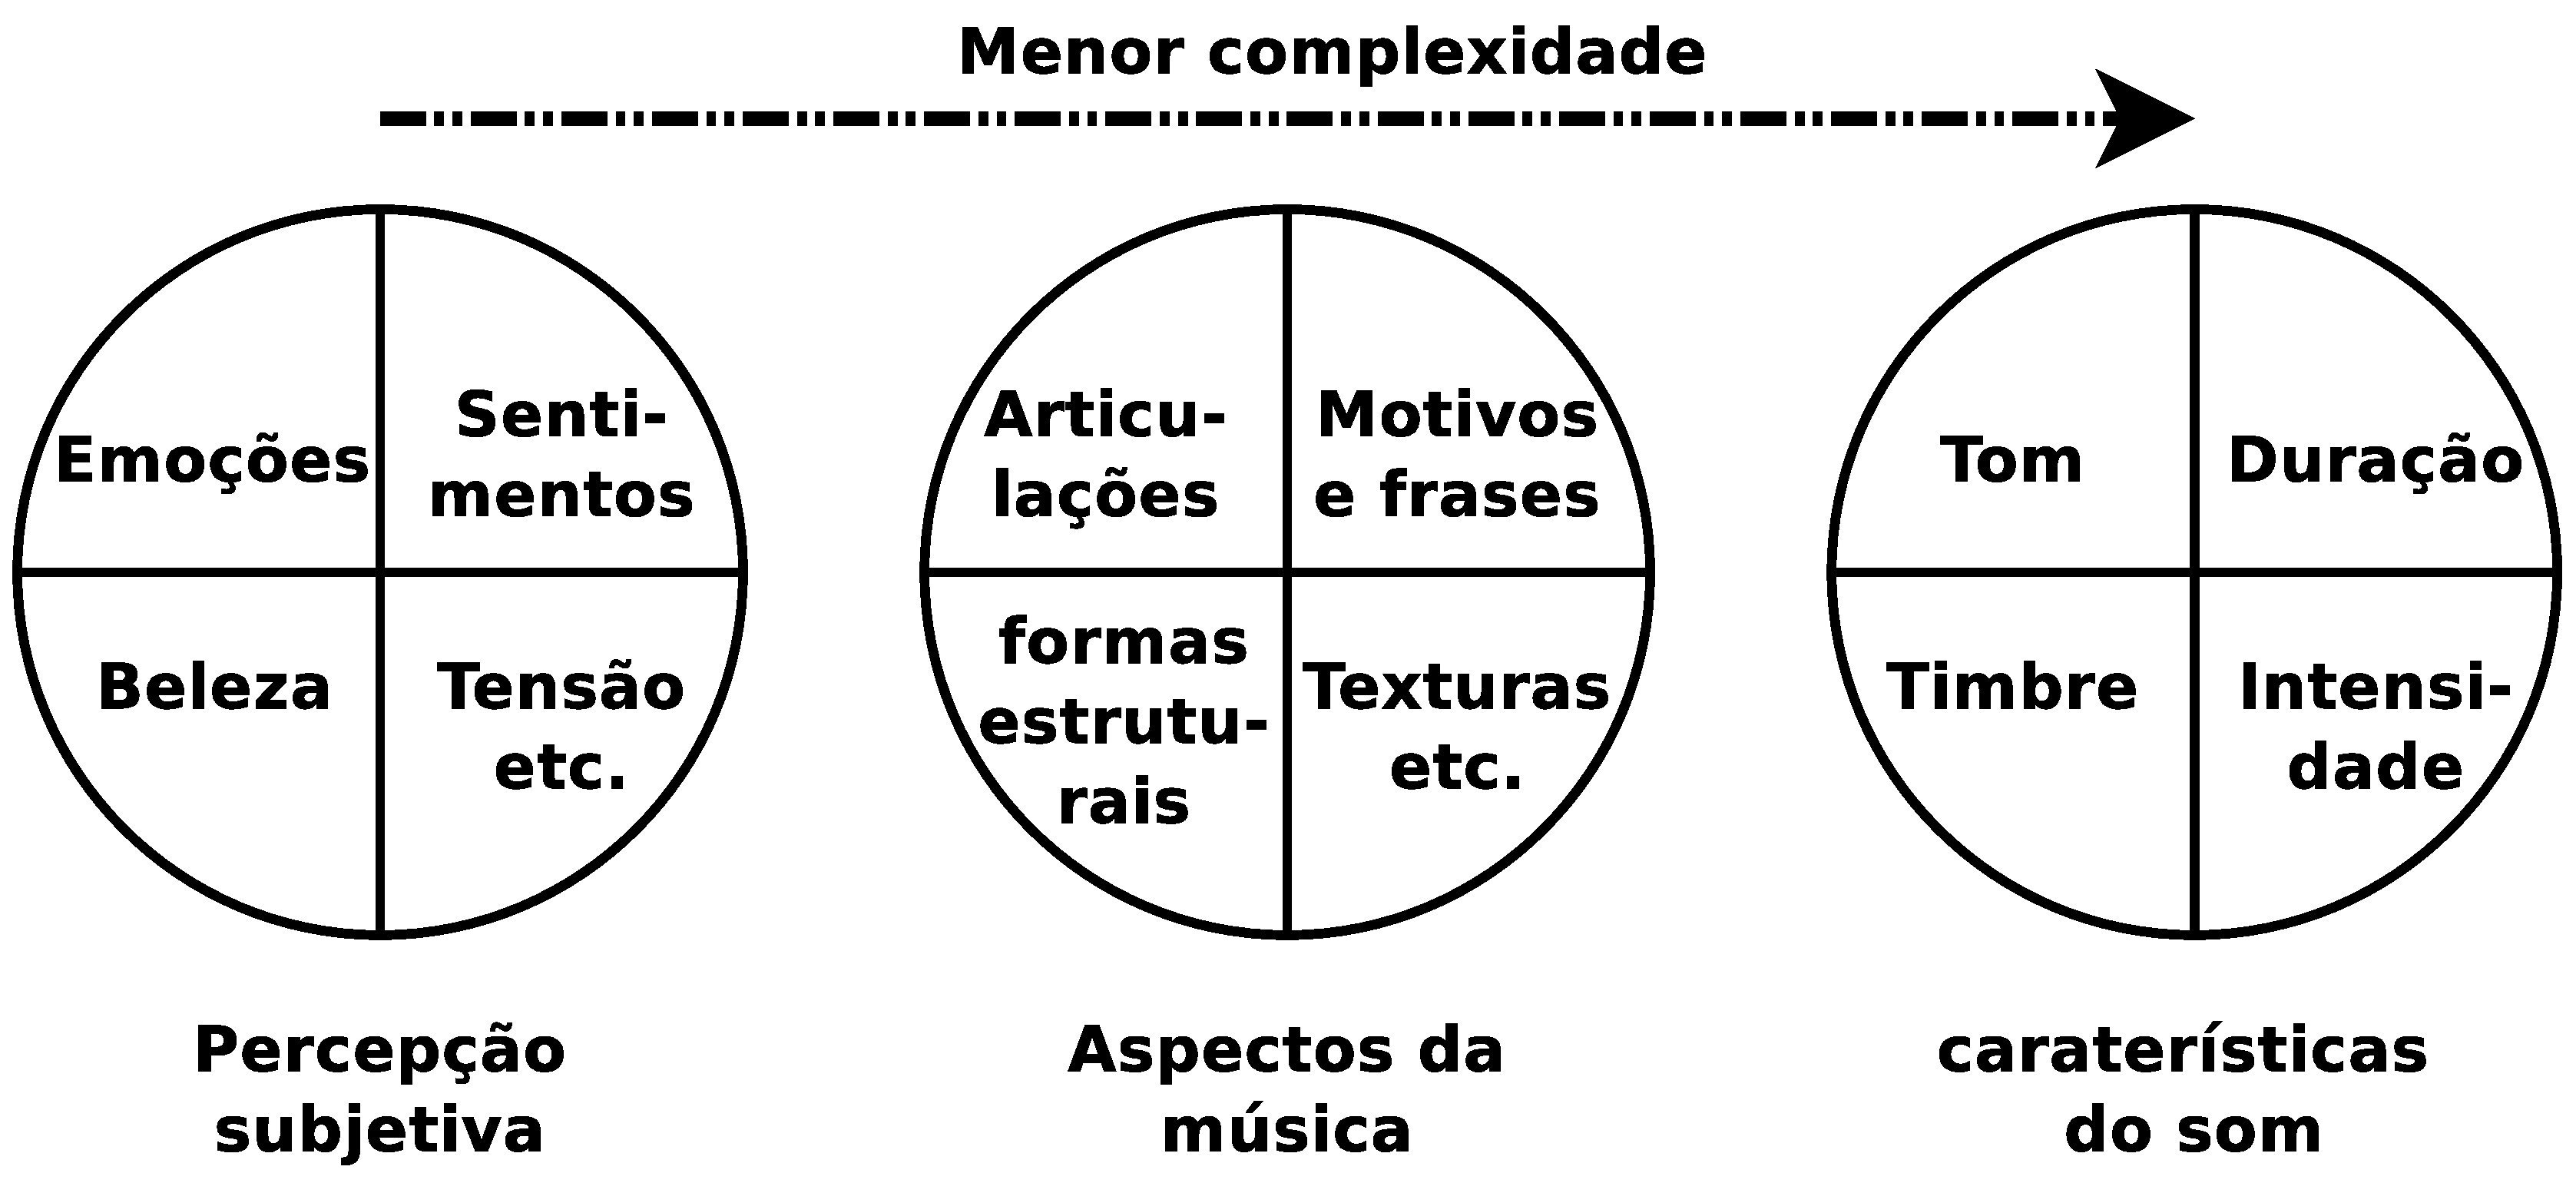
\includegraphics[width=\textwidth]{chapters/cap-musicalidade-tecnica/etapa-melodica-1.eps}
    \caption{Níveis de aproximação à música.}
    \label{fig:etapa-melodica-1}
\end{figure}

A continuação descreveremos como abordar na nossa dança o uso de uma melodia,
em todos os níveis de aproximação à música mostrados na Figura \ref{fig:etapa-melodica-1}.

%%%%%%%%%%%%%%%%%%%%%%%%%%%%%%%%%%%%%%%%%%%%%%%%%%%%%%%%%%%%%%%%%%%%%%%%%%%%%%%%
\subsubsection{Trabalhando as caraterísticas do som na melodia} 
Na 
Seção \ref{sec:elementosmusica} estudamos as \hyperref[sec:carateristasom]{\textbf{4 características do som}};
a nível de estudo da musicalidade, 
3 destas características já foram aproveitadas quando definimos \hyperref[subsec:dancaritmo]{\textbf{dançar no ritmo}};
sendo estas: 
\hyperref[sec:pos:Duracion]{\textbf{duração}}, 
\hyperref[sec:pos:Intensidade]{\textbf{intensidade}} e 
\hyperref[sec:pos:timbre]{\textbf{timbre}};
pelo que o aproveitamento destas caraterísticas não será descrito aqui\footnote{\label{footn:melodiatemritmo}Dançar 
na melodia envolve também \hyperref[subsec:dancaritmo]{\textbf{dançar no ritmo}}, 
pois toda melodia tem ritmo; 
porem, nesta seção quando falemos de dançar na melodia, 
só serão abordados aspectos da musicalidade não tratados em estagios anteriores.}.
A este nível de complexidade a única caraterística não usada é 
\{o \hyperref[sec:pos:Altura]{\textbf{tom}}\},
ou mais especificamente a mudança de \hyperref[sec:pos:Altura]{\textbf{alturas}} nas figuras musicais.

Porem, neste ponto devemos ter cuidado, 
pois seguir literalmente as mudanças de tom (altura)
seria mais próximo a \hyperref[subsubsec:musicvisualization]{\textbf{visualização musical}},
 ou a \hyperref[sec:mikeymousing]{\textbf{mickey mousing}}\footnote{Técnicas 
muito boas porem muito fáceis de virar enjoativas se são empregadas desnecessariamente.}.


\begin{example}[Seguindo o tom:] 
\label{ex:musicalidade:melodia:dtons}
Para interpretar as mudanças de tom, 
poderíamos realizar um movimento relativo\footnote{É usada a palavra ``relativo'',
pois não tem necessariamente que ser um movimento ascendente para representar um aumento de tom;
e sim, podemos digerir a ideia e mapear algum outro movimento; 
como por exemplo ir aos lados com movimentos longos.} 
a subir quando o tom aumenta,
e um relativo a descer quando o tom diminui.
\end{example}

Tecnicamente falando, 
fazer um hipotético e literal sobe e desce no Exemplo \ref{ex:musicalidade:melodia:dtons}, 
seria sim dançar na melodia\footnote{Seguir o as mudanças de tom com o corpo, 
de forma literal em todo momento, 
pode levar muito possivelmente a ter uma dança a principio engraçada e logo enjoativa.};
porem, 
existem outras caraterísticas relativas a mudanças de tom na melodia que podemos aproveitar. 

Como já foi estudado da Seção \ref{sec:caracteristicas:melodia},
podemos extrair pelo menos 3 características da melodia,
se analisamos esta em função das mudanças de tom;
estas caraterísticas são:
\{Extensão, Contorno, Movimento\}.
 
\begin{itemize}
\item \textbf{Dançando usando a extensão melódica:}
Melodias com uma \hyperref[ref:melodica:range]{\textbf{extensão melódica}} 
pequena nos produzem geralmente um clima de calma ou quietude;
por outro lado extensões maiores nos produzem geralmente uma sensação de liberdade e expansividade
 \cite[pp. 43]{holland2013music}.
Pelo que, para estar em comunião com a melodia, nossos movimentos deveriam acompanhar estas percepções.
\begin{example}[Usando o rango melódico:]
Na composição musical titulada ``Corcovado''  de Antônio Carlos Jobim,
podemos observar que esta tem uma forma $ABAC$\footnote{Com uma coda de 3 ou 4 compassos, dependendo da versão.},
com seções de 8 compassos binários cada um \cite{partituracorcovado1} \cite[pp. 53]{colluraimprovisacao}.

Ao escutar esta melodia, percebemos que as seções $A$ e $B$ tem uma extensão melódica pequena,
em comparação a seção $C$ que tem uma extensão melódica maior. 
Podemos identificar facilmente a seção $C$, pois a letra que acompanha a seção diz:
``E eu que era triste, descrente desse mundo, ao encontrar você eu conheci ...''.

Assim uma sugestão de interpretação, 
poderia ser usar movimentos com uma extensão pequena e contida para
a seção $A$ e $B$; e movimentos de percorrido mais amplo na seção $C$. 
\end{example}
\item \textbf{Dançando usando o contorno melódico:}
Quando conseguimos perceber o \hyperref[ref:melodica:shape]{\textbf{contorno}} de uma melodia,
podemos usar esta informação para visualizar mentalmente uma curva $f(t)$, em função do tempo $(t)$;
assim, podemos atrelar $f(t)$ a algum movimento ou \hyperref[sec:musicalidade:dinamicas]{\textbf{dinâmica}}.
\begin{example}[Usando a curva $f(t)$:]
Como já foi adiantado no Exemplo \ref{ex:musicalidade:melodia:dtons},
 os valores $f(t)$ podem ser usado em nossos movimentos; 
a continuação listamos algumas alternativas de uso.
\begin{itemize}
\item Distancia percorrida no salão em função de $f(t)$.
\item O espaço ocupado por nosso corpo ao realizar nossos movimentos em função de $f(t)$.
Por exemplo, se este valor é alto usamos um movimento que expanda as pernas como um ``Romário'',
ou um que expanda o espaço do \hyperref[def:Par]{\textbf{par de dança}}, como no ``assalto'', 
e se o valor de $f(t)$ é pequeno poderíamos usar movimentos no lugar usando um 
\hyperref[def:abracodedanca]{\textbf{abraço de dança}} fechado. 
\item \hyperref[subsec:dinamica:velocidade]{\textbf{Velocidade}} de nossos movimentos em função de $f(t)$.
\item \hyperref[sec:musicalidadetensionrelease]{\textbf{Tensão e relaxação}} de nosso corpo em função de $f(t)$.
\item etc.
\end{itemize}

Além de todas estas possibilidades, poderíamos fazer combinações e intercalar ou uso  destas escolhas.
\end{example}

\item \textbf{Dançando usando o movimento melódico:}
Quando vimos o tema da \hyperref[ref:melodica:range]{\textbf{extensão melódica}},
quantificamos às melodias em função da distancia entre a nota musical mais alta e a mais baixa;
este critério nos deu a possibilidade de projetar nossa dança entre dois extremos,
livre e contido, respetivamente;
porem este tipo de avaliação é um parecer promédio,
para a melodia ou uma porção dela. 
Assim, se escolhemos um movimento como deslocar-nos numa direção 
para interpretar a \hyperref[ref:melodica:range]{\textbf{extensão melódica}} numa porção de melodia,
observaremos que precisamos de um critério que nos indique como serão os sub-movimentos para completar esta ação;
este critério pode ser completado se usamos o analises do \hyperref[ref:melodica:movimento]{\textbf{movimento melódico}},
para escolher as dinâmicas dos submovimentos.
\begin{example}[Usando o movimento melódico:]
Se percebemos que a melodia esta composta por movimentos melódicos conjuntos;
então, 
os sub-movimentos de nossa dança poderiam ser executados realizando mudanças pequenas ou deslocamentos curtos,
por outro lado se percebemos movimentos melódicos disjuntos,
os sub-movimentos de nossa dança poderiam ser executados realizando mudanças grandes ou deslocamentos longos.
\end{example}
\end{itemize}


%%%%%%%%%%%%%%%%%%%%%%%%%%%%%%%%%%%%%%%%%%%%%%%%%%%%%%%%%%%%%%%%%%%%%%%%%%%%%%%%
\subsubsection{Trabalhando os aspectos da música na melodia} 
Quando analisamos a música desde um ponto de vista mais técnico, 
podemos extrair desta varias caraterísticas; 
neste sentido, nos Capítulos \ref{cap:musicabasica},
\ref{cap:musicacomposer} e \ref{cap:musicatopicos},
foram apresentadas algumas características da música, 
descritas desde o ponto de vista do compositor musical;
por outro lado, no Capítulo \ref{cap:percepcaomusical} 
foram abordados alguns aspectos da música desde o ponto de vista da percepção de um ouvinte.
Assim, juntando estas duas visões da música,
podemos formar um critério para interpretar  na nossa dança um componente da música, como a melodia.
A seguir listaremos algumas sugestões sobre escolhas criativas para interpretar a melodia na nossa dança.

Uso de dinâmicas sobre a melodia. 
\begin{itemize}
\item Motivos (leitmotiv); Uso de motivos ou ideias melódicas: Escolher um motivo, ou ideia melódica pequena e dar um passo no final, 
aplicando uma dinâmica em concordância com a ideia melódica.
\item Frases (cadências).
\item Fraseio da linha melódica.
\item Articulações
\item Formas estruturais.
\end{itemize}



%%%%%%%%%%%%%%%%%%%%%%%%%%%%%%%%%%%%%%%%%%%%%%%%%%%%%%%%%%%%%%%%%%%%%%%%%%%%%%%%
\subsubsection{Trabalhando nossa interpretação subjetiva da melodia} 

Você precisará se concentrar na qualidade expressão emocional da linha melódica.

Melodia não pode existir sem ritmo, mas acrescenta emoção, doçura e continuidade à música.

Melodia é o que faz com que nossos passos para se tornar elegante, 
graciosa, sentimental e persistente, enquanto tentamos expressar a beleza, emoção e fluidez da melodia.


\begin{itemize}
\item eu sigo a intensidade da mesma.
\end{itemize}

%%%%%%%%%%%%%%%%%%%%%%%%%%%%%%%%%%%%%%%%%%%%%%%%%%%%%%%%%%%%%%%%%%%%%%%%%%%%%%%%
\subsubsection{Exemplos} 

Para darle un poco más de libertad y creatividad, 
mantener el pulso o el ritmo en sus pies le brinda la capacidad de interpretar 
la melodía con el resto de su cuerpo ou realizando dinâmicas, si así lo desea.



%%%%%%%%%%%%%%%%%%%%%%%%%%%%%%%%%%%%%%%%%%%%%%%%%%%%%%%%%%%%%%%%%%%%%%%%%%%%%%%%
%%%%%%%%%%%%%%%%%%%%%%%%%%%%%%%%%%%%%%%%%%%%%%%%%%%%%%%%%%%%%%%%%%%%%%%%%%%%%%%%
\subsection{\textcolor{red}{Dançar na música}}
\label{subsec:dancamusica}
\index{Musicalidade!Dançar na música}

nesse sentido na Seção \ref{sec:elementosmusica} foram listados,
os elementos da música, sendo estes:
\begin{inparaitem}
\item \hyperref[sec:pos:Ritmo]{\textbf{Ritmo}}
\item \hyperref[sec:pos:Melodia]{\textbf{Melodia}}
\item \hyperref[sec:pos:Harmonia]{\textbf{Harmonia}}
\item \hyperref[sec:pos:Contraponto]{\textbf{Contraponto}}
\end{inparaitem}

%%%%%%%%%%%%%%%%%%%%%%%%%%%%%%%%%%%%%%%%%%%%%%%%%%%%%%%%%%%%%%%%%%%%%%%%%%%%%%%%
%%%%%%%%%%%%%%%%%%%%%%%%%%%%%%%%%%%%%%%%%%%%%%%%%%%%%%%%%%%%%%%%%%%%%%%%%%%%%%%%
%%%%%%%%%%%%%%%%%%%%%%%%%%%%%%%%%%%%%%%%%%%%%%%%%%%%%%%%%%%%%%%%%%%%%%%%%%%%%%%%
\begin{comment}

\subsection{Emoções vs. sentimentos}
\label{ref:emotionsentimental}
Mesmo que sejam tratados como similares, 
existem diferencias entre as emoções e os sentimentos.
Por exemplo é sabido que:
\begin{itemize}
\item Alguns sentimentos estão relacionados com as emoções especificas \cite{freitas2015codigo} \cite[pp. 32]{nicolas2018musicas}.
\item Todas as emoções provocam sentimentos, porem não todos os sentimentos provem de emoções
\cite[pp. 288]{zanelli2014psicologia} \cite{freitas2015codigo}.
\item Os sentimentos podem provocar emoções \cite{freitas2013psicologia}.
\item As emoções a diferença dos sentimentos podem ser fingidos ou genuínos \cite[pp. 32]{nicolas2018musicas}.
\item As emoções são a reação a um estimulo, enquanto que os sentimentos vem de um processo cognitivo \cite{freitas2013psicologia}.
\end{itemize}

\subsubsection{As emoções} 
São fenômenos complexos e com múltiplas dimensões,
sendo a emoção uma resposta automática, rápida, de curta vida e intensa, 
que pode chegar a nos de forma consciente ou inconsciente;
sendo este um impulso neuronal que provoca no organismo a execução de uma ação,
como comportamentos de aproximação ou afastamento
\cite[pp. 288]{zanelli2014psicologia}  \cite{freitas2015codigo}.
As funções da emoção estão ligadas à adaptação e à expressão, 
sendo este um catalisador entre nossa conduta e o meio que nos embrulha;
as emoções também cumprem um papel importante no desenvolvimento da aprendizagem 
(reforços positivos ou negativos)
  \cite{freitas2015codigo},
e permite a articulação social, política e cultural dos afetos \cite[pp. 32]{nicolas2018musicas}.

As emoções básicas no ser humano são \cite{freitas2015codigo} \cite[pp. 291]{zanelli2014psicologia}:
\begin{inparaitem}
\item felicidade (alegria)  % \cite{freitas2015codigo} \cite[pp. 291]{zanelli2014psicologia}
\item tristeza              % \cite{freitas2015codigo} \cite[pp. 291]{zanelli2014psicologia}
\item repugnância (aversão) % \cite{freitas2015codigo} \cite[pp. 291]{zanelli2014psicologia}
\item surpresa              % \cite{freitas2015codigo} \cite[pp. 291]{zanelli2014psicologia}
\item medo                  % \cite{freitas2015codigo} \cite[pp. 291]{zanelli2014psicologia}
\item raiva (cólera)        % \cite{freitas2015codigo}
\item desprezo              % \cite{freitas2015codigo}
\end{inparaitem}.

Os componentes da emoção são \cite[pp. 26]{redorta2006emocion} \cite{freitas2015codigo} \cite{freitas2013psicologia} :
\begin{description}
\item[Vivencia consciente:] (Ou componente cognitiva) Sensações que as pessoas vivenciamos subjetivamente.
Podemos sentir medo, angustia, raiva, entre outros.
Por exemplo, uma criança ao ver um palhaço pode provocar-lhe alegria, ou medo,
sendo este resultado subjetivo a cada pessoa. 
\item[Reações fisiológicas:] (Ou componente neurofisiológica) Órgão e sistemas emergentes da atividade emocional.
este se manifesta com respostas ``involuntárias'' como: 
taquicardia, 
sudoração, 
vasoconstrição, 
hipertensão, 
mudanças no tom muscular,
rubor, 
sequidade na boca, 
secreções corporais, 
etc.
\item[Comportamento expressivo:] (Ou componente conductual) 
Como as pessoas expressam essas emoções de forma verbal e não verbal.
No caso da forma verbal, podem ser percebidas, mudanças do tom na voz, no volumem, no ritmo, entre outros;
e no caso da forma não verbal, podemos observar mudanças na forma como o corpo se movimenta,
como um andar erguido ou encovado, lento ou rápido, etc.

\end{description}


%% \cite{freitas2015codigo}
%% \begin{itemize}
%% \item A cognição
%% \item a expressão facial
%% \item atividades do sistema nervoso autônomo (SNA)
%% \end{itemize}


\subsubsection{Os sentimentos} 
São um ``processo cognitivo'' 
de acompanhamento continuo de uma experiencia subjetiva, 
que pode ser provocada, ou não, por emoções \cite[pp. 288]{zanelli2014psicologia} \cite{freitas2013psicologia}.
Assim, podemos separar os sentimentos em dois categorias \cite[pp. 288]{zanelli2014psicologia}:
\begin{itemize}
\item Os sentimentos provocados por emoções, proveniente de alterações corporais.
Sendo estes sentimentos um juízo, ou procesamento, que fazemos sobre as emoções. 
\item Os sentimentos de fundo, este é originado pela existência humana.
\end{itemize}


\end{comment}

